\documentclass[12pt]{article}
\usepackage{amsmath}
\usepackage{amssymb} %mathbb
\usepackage{graphicx}
\usepackage{hyperref}
\usepackage[latin1]{inputenc}
\usepackage[top=1.0cm,bottom=1.3cm,left=1.0cm,right=1.0cm]{geometry}

\begin{document}

\Large

\begin{center}
Resum\~ao do Ogata
\end{center}

\normalsize

OGATA, K. Engenharia de Controle Moderno. Quinta Edi\c{c}\~ao em portugu\^es dispon\'ivel na livraria russa submundial.

\vspace{3mm}

Mundo n\~ao linear.

$u$ \'e entrada. $x$ \'e vari\'avel intermedi\'aria. $y$ \'e sa\'ida.

		\begin{center}
		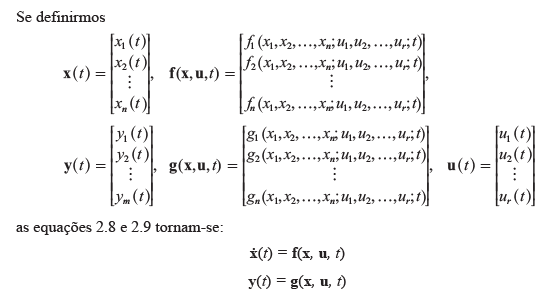
\includegraphics{26}
		\end{center}

Lineariza\c{c}\~ao.

		\begin{center}
		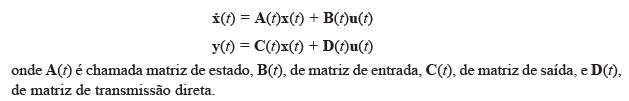
\includegraphics{27}
		\end{center}

Pelo mesmo m\'etodo de varia\c{c}\~ao de par\^ametros de E.D.O., ordem en\'esima vira ordem $1$.

Divida a transformada de Laplace da sa\'ida $\mathcal{L}(y)$ pela da entrada $\mathcal{L}(u)$ em fun\c{c}\~ao da vari\'avel $s$. Essa fun\c{c}\~ao $G(s)$ \'e chamada fun\c{c}\~ao de transfer\^encia do sistema din\^amico.

O autor fala de proporcional, integrador e derivador, depois junta tudo. A primeira vez que isso \'e bem explicado \'e na p\'agina $111$.

		\begin{center}
		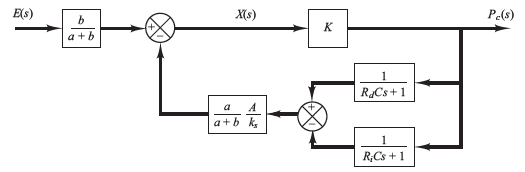
\includegraphics{111}
		\end{center}

		\begin{center}
		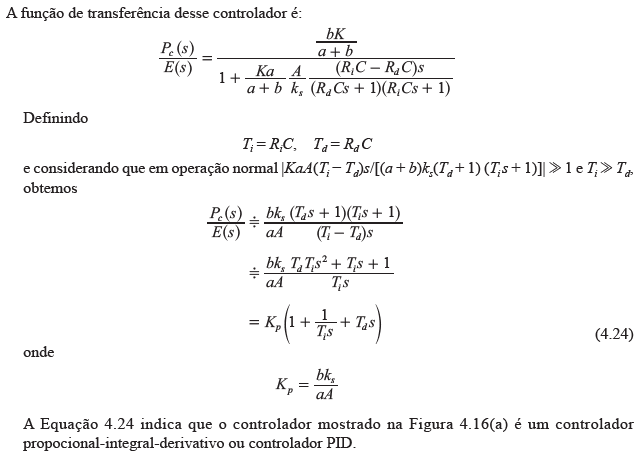
\includegraphics{110}
		\end{center}

Isso a\'i d\'a na mesma se \'e mec\^anico, el\'etrico, flu\'idico, t\'ermico, pneum\'atico, hidr\'aulico.

E o s\'olido. Na copasa, junto com os gases e os l\'iquidos, h\'a v\'alvulas para s\'olidos tamb\'em, uai.

Foi isso mesmo que voc\^e viu! O cara cancela $\cfrac{a}{1 + b} := \cfrac{a}{b}$, depois cancela $T_d$ perto de $T_i$, mas perto do inverso de $T_i$, o termo \'e considerado.

O cap\'itulo $5$ \'e an\'alise de ordem. Explica por que todas as outras ordens devem ser descartadas. E voltamos \`a primeira ordem no cap\'itulo $6$. Parei na p\'agina 246.

N\~ao tem como resumir mais. Se o engenheiro n\~ao quer propor\c{c}\~ao, zera as constantes $P\sim O(s^0)$. Se n\~ao quer integra\c{c}\~ao, zera as constantes $I\sim O(s^{-1})$. Se n\~ao quer deriva\c{c}\~ao, zera as constantes $D\sim O(s^1)$.

\vspace{3mm}

Fora da caridade, n\~ao h\'a salva\c{c}\~ao. Com caridade, h\'a evolu\c{c}\~ao.

Vinicius Claudino Ferraz, vers\~ao $0.1$ de $7$/mar/$2020$.

\end{document}
